\section{The Dependence of Number of Particles on Radial Distribution}
\label{sec:NumberPartRadDist}
\tabref{tab:NumberPartRadDist} shows the dependence of number of particles on the average distance to the cluster center after reached equilibrium. 
From the table it seems that the final distance might be slightly increased when the number of particles increases. 
However, then is not a strong tendency. 
\begin{table}[H]
\centering
\begin{tabular}{|c|c|}
\hline
Number of particles  & Mean distance to center (ly)  \\
\hline
30 & 12.36
\\ \hline
50 & 13.69
\\ \hline
70 & 13.11
\\ \hline
100 & 14.75
\\ \hline
200 & 14.08
\\ \hline
\end{tabular}
\caption{
The average distance to the cluster center of bound particles after $3\tau_{crunch}$ with a step length of $10^{-4}\tau_{crunch}$ and $\epsilon = 10^{-7}$ for different numbers of particles bot same total mass.
}
\label{tab:NumberPartRadDist}
\end{table}
\begin{figure}[H]
\centering
\begin{minipage}{.5\textwidth}
  \centering
  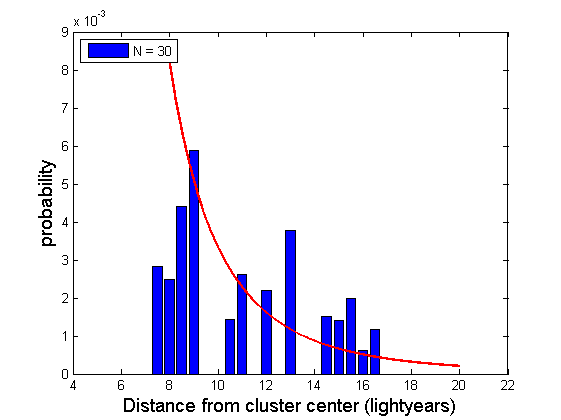
\includegraphics[width=1\linewidth]{Figures/N30.png}
\end{minipage}%
\begin{minipage}{.5\textwidth}
  \centering
  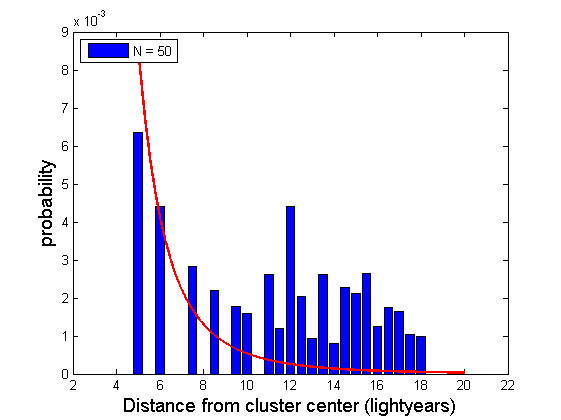
\includegraphics[width=1\linewidth]{Figures/N50.png}
\end{minipage}
\begin{minipage}{.5\textwidth}
  \centering
  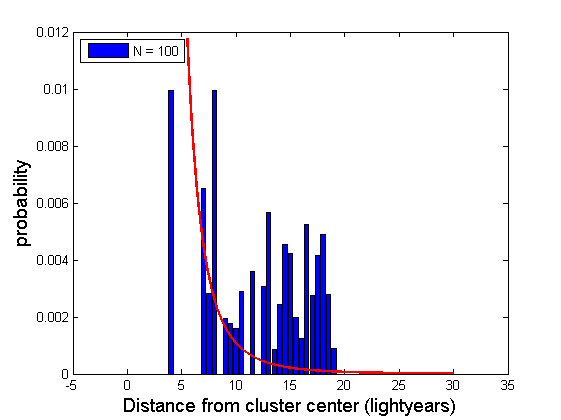
\includegraphics[width=1\linewidth]{Figures/N100.png}
\end{minipage}%
\begin{minipage}{.5\textwidth}
  \centering
  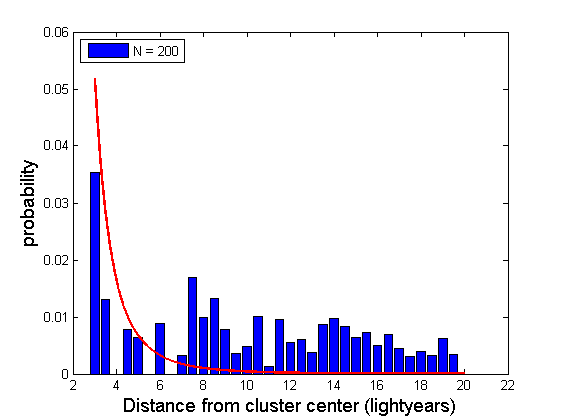
\includegraphics[width=1\linewidth]{Figures/N200.png}
\end{minipage}
\caption{
Radial density of bound particles after a time period of $3\tau_{crunch}$ plotted together with a fit computed from \matref{eq:radialDens}.
}
\label{fig:NumberPartRadDist}
\end{figure}
The histograms in \figref{fig:NumberPartRadDist} show the radial particle density for N = 30, 50, 100 and 200 (see \tabref{tab:NumberPartRadDist}).
The radial density is found by counting the number of particles at a distance $r_i$ from the center and dividing this by the sphere area, given as $4\pi r_i^2$ at this point, multiplied by the interval $dr$ that corresponds to the thickness of the bars in the histograms. 
The red curves are made to fit the radial density from the formula
\begin{align}
	n(r) = \frac{n_0}{\left( 1 0+ \left( \frac{r}{r_0} \right) ^4 \right)}
	\label{eq:radialDens}
	\end{align}
in which $n_0 \propto N^2$ and $r_0 \propto N^{-1/3}$
 \cite{ColdUniformSphericalCollapse}. 
The fit is not perfect, especially not for longer distances from the cluster center. 
However, the computed radial densities follow the appearance of the simple expression in \matref{eq:radialDens}.